\documentclass[letterpaper,12pt]{article}
\usepackage[utf8]{inputenc}
\usepackage{fullpage}
\usepackage{courier}
\usepackage[margin=0.75in]{geometry}
\usepackage{listings}
\usepackage{color}
\usepackage{graphicx}
\usepackage[width=4in]{caption}
\usepackage{hyphenat}

% Format a sectionless paragraph
\newcommand*\unparagraph{
	\par
	\nopagebreak
	\vskip3.25ex plus1ex minus.2ex
	\noindent
}

% define extra colors
\definecolor{dkgreen}{rgb}{0,0.6,0}
\definecolor{purple}{RGB}{159,0,197}

% define the code listing format
\lstset{
	language=C++,
	basicstyle=\ttfamily,
	backgroundcolor=\color{white},
	showspaces=false,
	showstringspaces=false,
	frame=none,
	tabsize=3,
	keywordstyle=\color{purple},
	commentstyle=\color{dkgreen},
	stringstyle=\color{blue},
	escapeinside={\%*}{*)}
}

% Define the title/header
\title{\Large CS 1428\\Lab 8 Sections L06 and L19} 
\author{Jared Wallace}
\date{}

\begin{document}

\maketitle

\section*{1-D Arrays and Character Arrays}
1 dimensional arrays and character arrays (often called ``C-strings'') are good examples
of the different types of array processing you will encounter.  The first example is when 
we know the size of the array (I hope a bell just rang in your head about which loop to use).

Using a for loop with the size of the array as the limit will allow us to visit each element 
of the array one at a time and do whatever we want to with it.

% code example here
\begin{lstlisting}[basicstyle=\footnotesize\ttfamily]
const int SIZE = 15;
int arr[SIZE];

for (int i = 0; i < SIZE; ++i)
	cout << arr[i] << " \n";

\end{lstlisting}

C-strings utilize what is known as a sentinel value, specifically a null character ('\textbackslash{}0').  With
a while loop we can watch for that null terminator and know when to stop.

% code example here
\begin{lstlisting}[basicstyle=\footnotesize\ttfamily]
char arr[] = "C-string";          // [`C' `-' `s' `t' `r' `i' `n' `g' `\0']
int index = 0;

while(arr[index] != `\0') {
	cout << arr[index];
	index++;
}

// This can also be done with a for loop
for(int i = 0; arr[i] != '\0'; ++i)
	cout << arr[i];
\end{lstlisting}

\section*{C Strings}
I want you to declare a C-string with the contents "I am a C-string".  You will create several
new strings that contain manipulations of this original string but at the end of the program this
string should be still intact. You might find it helpful to declare a constant that holds the size
of the array.  You may NOT use this size as a limit when there is a sentinel value but it will be
useful for declaring new arrays. Each of the following tasks should be performed on the original
string, not on the result of the previous task.

\begin{enumerate}
	\item First I want you to create a new copy of the string that is in reverse.  Recall that to be a valid 
	C-string the null terminator (which is not considered part of the content) must be at the end of the
	string before we declare the operation complete.

	\item Recall during the discussion of switch statements when we discussed that characters are stored in the
	computer as integers. When you assign a character to an integer the integer takes the value of that 
	ASCII value.  Create an integer array (SIZE - 1 since there is no null terminator) that contains the
	integer values of each character.

	\item By checking the if the integer value of a particular character is within a certain range $97 \le $ char $ \le 122$
	we can determine if it is a lowercase character.  We can then convert it to uppercase by subtracting 32
	to that value. Visit each item in the original array and set the corresponding positions in a new array 
	with the upper-case character that corresponds.
\end{enumerate}

Print each of these arrays out to the screen in readable format including labeling what each one is.

% Don't forget the submission instructions!
\unparagraph{} \textbf{Upload your source code through the homework upload utility.  Place a printout
of you source code behind this page and staple before turning it in at my desk}

\vspace{20mm}

% Comic at the bottom
\begin{figure}[ht!]
	\centering
	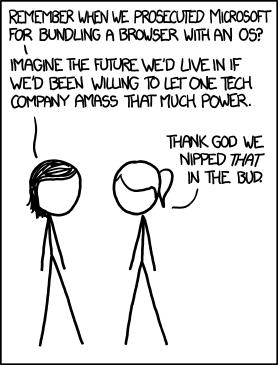
\includegraphics[width=3in]{microsoft.png}
	\caption*{Facebook, Apple, and Google all got away with their monopolist power grabs because they don't have
	any S's in their names for critics to snarkily replace with \$'s}
\end{figure}

\end{document}
